\clearpage
\subsection{premi/client}
\begin{figure}[h]
\begin{center}
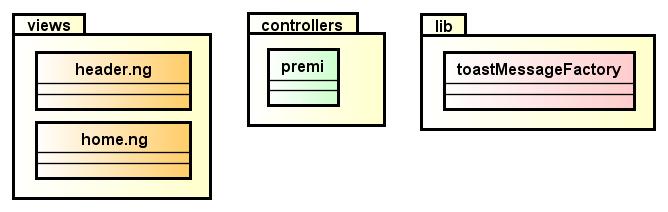
\includegraphics[scale=0.50]{img/diapkg/client.png}
\caption{Diagramma del package premi/client}
\end{center}
\end{figure}



%-------  diagramma di un template %
\subsubsection{premi/client/views/container.ng}

\begin{description}
%-------  descrizione del template%
\item[Descrizione] \hfill
	Semplice contenitore utilizzato da altri template per la creazione di viste nell'applicazione
\end{description}



%-------  diagramma di un template %
\subsubsection{premi/client/views/fluidContainer.ng}

\begin{description}
%-------  descrizione del template%
\item[Descrizione] \hfill
	Semplice contenitore utilizzato da altri template per la creazione di viste nell'applicazione
\end{description}



%-------  diagramma di un template %
\subsubsection{premi/client/views/header.ng}

\begin{description}
%-------  descrizione del template%
\item[Descrizione] \hfill
	Template che genera un header per la pagina principale dell'applicazione
	\item[Note] \hfill
	\begin{itemize}
			\item Deve mostrare il nome dell'utente, se loggato, oppure un pulsante per loggarsi
			\item Deve mostrare un pulsante per accedere alla pagina di modifica della passsword, se l'utente è loggato
	\end{itemize}
\end{description}

%-------  diagramma di un template %
\subsubsection{premi/client/views/home.ng}

\begin{description}
%-------  descrizione del template%
\item[Descrizione] \hfill
	Template della principale dell'applicazione
	\item[Note] \hfill
	\begin{itemize}
			\item Deve mostrare il logo dell'applicazione
			\item Deve mostrare un pulsante per registarsi, se l'utente non è loggato
	\end{itemize}
\end{description}

%-------  diagramma di un template %
\subsubsection{premi/client/controllers/premi}

\begin{description}
%-------  descrizione del template%
\item[Descrizione] \hfill
	Controller della pagina principale dell'applicazione. Rende \textit{currentUser} "reattivo", ossia utilizza il metodo getReactively di urigo:angular-meteor$_G$ per fare in modo che venga inviato un segnale ogni volta che currentUser cambia
\end{description}

%-------  diagramma di un template %
\subsubsection{premi/client/lib/toastMessageFactory}

\begin{description}
%-------  descrizione del template%
\item[Descrizione] \hfill
	Semplice factory che restituisce una funzione per l'invio di notifiche o messaggi di errore all'utente
\end{description}

